\documentclass[german]{scrartcl}
\usepackage[ngerman]{babel}
\usepackage[babel,german=quotes]{csquotes}

\usepackage{paper}

\author{Moritz Marc Beller \& Fabian Streitel \\ Technische Universität München}
\title{Masterpraktikum im Wintersemester 2011 \\
Open-Source Praktikum \\
\textit{Ein Mapeditor für Unknown Horizons}}
\date{\today} % TODO adjust?

\begin{document}
\maketitle{}

\section{Einleitung}
Ein integraler Bestandteil eines jeden größeren Computerspiels ist die
Möglichkeit, effizient die Spielinhalte editieren zu können. Hierzu wird in vielen Spielen ein sogenannter Mapeditor verwendet.
Dieser ermöglicht es, die Dateien zu editieren, die die Spielinhalte enthalten, wie etwa
die Landschaft, Gebäude, Akteure und vieles mehr.
Ohne ein solches Werkzeug ist das gezielte Erstellen von Spielinhalten mühsam
oder gar völlig unmöglich.

\enquote{Unknown Horizons} (UH) \cite{uh} ist ein Open Source
Aufbaustrategiespiel nach dem Vorbild der Anno-Serie von Sunflowers.
Es ist
besonders interessant, da es nur wenige Open Source Spiele mit einer aktiven
Community und einem solchen Reifengrad gibt. Als Folge konnte UH drei Teilnehmer des
Google Summer of Code des Jahres 2011 für sich gewinnen.

Auch für Unknown Horizons ist ein Mapeditor im aktuellen Stadium von besonderer
Wichtigkeit.
Zwar kann das Spiel zufällige Karten generieren, dies genügt jedoch den
Ansprüchen des Spiels nicht mehr. Einerseits benötigen die Entwickler für
wiederkehrende Tests vorgegebene Karten mit bestimmten Eigenschaften.
Andererseits ist ein Editor für das gezielte Erstellen von statischen
Spielelementen, wie z.B. der kürzlich integrierte
Kampangenmodus, unabdingbar. Auch können nur so vorgegebene Karten mit einem
festgelegten Schwierigkeitsgrad erzeugt werden.

Im Folgenden beschreiben wir unser Vorgehen bei der Planung und Entwicklung
eines Mapeditors für UH. Hierzu geben wir zunächst einen detaillierteren
Überblick über UH und das Entwicklungsteam, das hinter dem Projekt steht.
Anschließend beschreiben wir die softwaretechnischen Aspekte der Implementierung, gefolgt
von einer Beschreibung unseres Vorgehens bei der Umsetzung der Software. Abschließend
geben wir unsere persönlichen Erfahrungen und Eindrücke zum Ablauf und Ergebnis des Projekts
wieder.



\section{Unknown Horizons und FIFE}
„Unknown Horizons“ (UH) \cite{uh} ist ein in Python geschriebenes Open Source Aufbaustra-
tegiespiel. Es basiert auf der in C++
verfassten FIFE Graphikengine. Die Ansicht ist isometrisch mit vorgerenderten 3D-Modellen,
die auf Kachel-basierten Karten dargestellt werden. Es wird circa alle drei Monate eine neue Version
veröffentlicht. Das aktuelle Projekt baut auf einer Reihe von Vorgängern auf, welche
in C++ geschrieben wurden, deren Entwicklung jedoch eingestellt ist.
% TODO cite!

\subsection{Die UH Community}
UH besitzt eine sehr aktive internationale Community von Entwicklern, Spieldesignern und Graphikern, die
sich der Weiterentwicklung und Verbesserung des Spiels widmen.
Es finden regelmäßig Treffen zum Brainstorming, Wochenrückblick
und zur Planung im IRC sonntäglich um 19.00 Uhr MEZ statt. Von diesen Meetings existieren
öffentliche Logs \cite{uhlogs}.
Diese Meetings dienen als Haupt-Kommunikationsmittel zwischen den einzelnen Projektteilnehmern,
es findet jedoch auch außerhalb der Meetingzeiten ein Austausch über den  IRC-Channel statt.
Dieser ist somit das
Hauptkommunikationsmittel des Projekt. Daneben existieren noch ein Forum
und eine Mailingliste. Das Projekt verwendet Git zur Versionskontrolle und Trac für
Bugtracking.
% TODO github

\subsection{Die Beziehung zwischen UH und FIFE}
Die \enquote{Flexible Isometric Free Engine} (FIFE) \cite{fife} ist eine in C++ geschriebenes Framework
zum Erstellen von verschiedenen Spieltypen. Sie dient als Grundlage von UH und übernimmt das Rendern
der Spielgrafik.

Die beiden Projekte sind zwar separat, jedoch besteht eine enge Beziehung zwischen ihnen. Zum einen
engagieren sich viele der UH Entwickler auch im FIFE Projekt und verbessern die Engine nach Bedarf.
Zum andern ist UH das Vorzeigeprojekt von FIFE, das als Demonstration der Engine hergenommen wird.



\section{Implementierung}
\subsection{Integration in die UH Codebase}
\subsubsection{Das Kartenformat}
\label{kartenformat}

%
% algorithm principle
%
\begin{figure}[htbp]
  \centering
  
    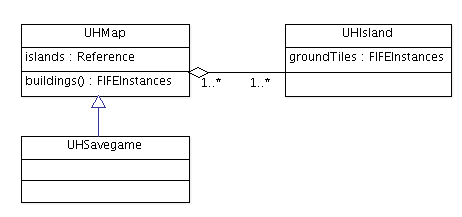
\includegraphics[width=0.7\textwidth]{gfx/klassendiagramm-UHSaveGame.png}
  
  \caption{UML Diagramm des Kartenformates von UH.}
  \label{figure:automaton-intersection}
\end{figure}

UHs Kartenformat im SQLite besteht grob aus den folgenden Elementen für den
Editor relevanten Elementen:
\begin{itemize}
  \item Allgemeinen Karteninformationen
  \item Die auf der Karte plazierten Objekte (wie Gebäude etc.)
  \item Verweise auf Island-Files. \\ 
  Ein Island-File ist eine SQLite-Datenbank,
  die die Informationen über die Bodenbeschaffenheit einer zusammengehörenden
  Inseln enthält:
  \begin{itemize}
    \item Allgemeine Islandinformationen
    \item Alle zu einem Island gehörenden Groundtiles
  \end{itemize}
\end{itemize} 

\subsection{Kommandozeilen-Parameter (FIFE)}
\subsection{Schaffung der Plugin-Infrastruktur (FIFE)}

\subsection{Plugin zum Laden von UH Objekten (UH)}
\subsection{Plugin zum Laden von UH Karten (UH)}
\subsection{Plugin zum Speichern von UH Karten (UH)}
Das Plugin zum Speichern weist die Schwierigkeit auf, dass der Editor nicht die
Interna des UH Spielmodells kennen kann. Der Editor ``zeichnet'' einfach nur
Elemente wie Bodentiles und Gebäude auf die verschiedenen Layer-Schichten, das
Saver-Plugin muss diese im UH-Modell speichern. 


Die Layer-Schichten enthalten vor dem Speichern die Instanzen aller vom User
gesetzen Gebäude und Bodentiles. 

Der Algorithmus geht dabei den Groundlayer vom Urpsrung des Koordinatensystems
Origo (0, 0) nach rechts unten ab. Durch diese Traversierungsstrategie muss nur
nach oben und nach links auf zu verbindenden Islands überprüft werden. Findet
sich ein direkt angrenzendes Groundtiles, so wird das akutelle Groundtiles (rot
hinterlegt) mit dem bestehenden vereinigt, indem es dessen Insel-ID übernimmt.

%
% algorithm principle
%
\begin{figure}[htbp]
  \centering
  
    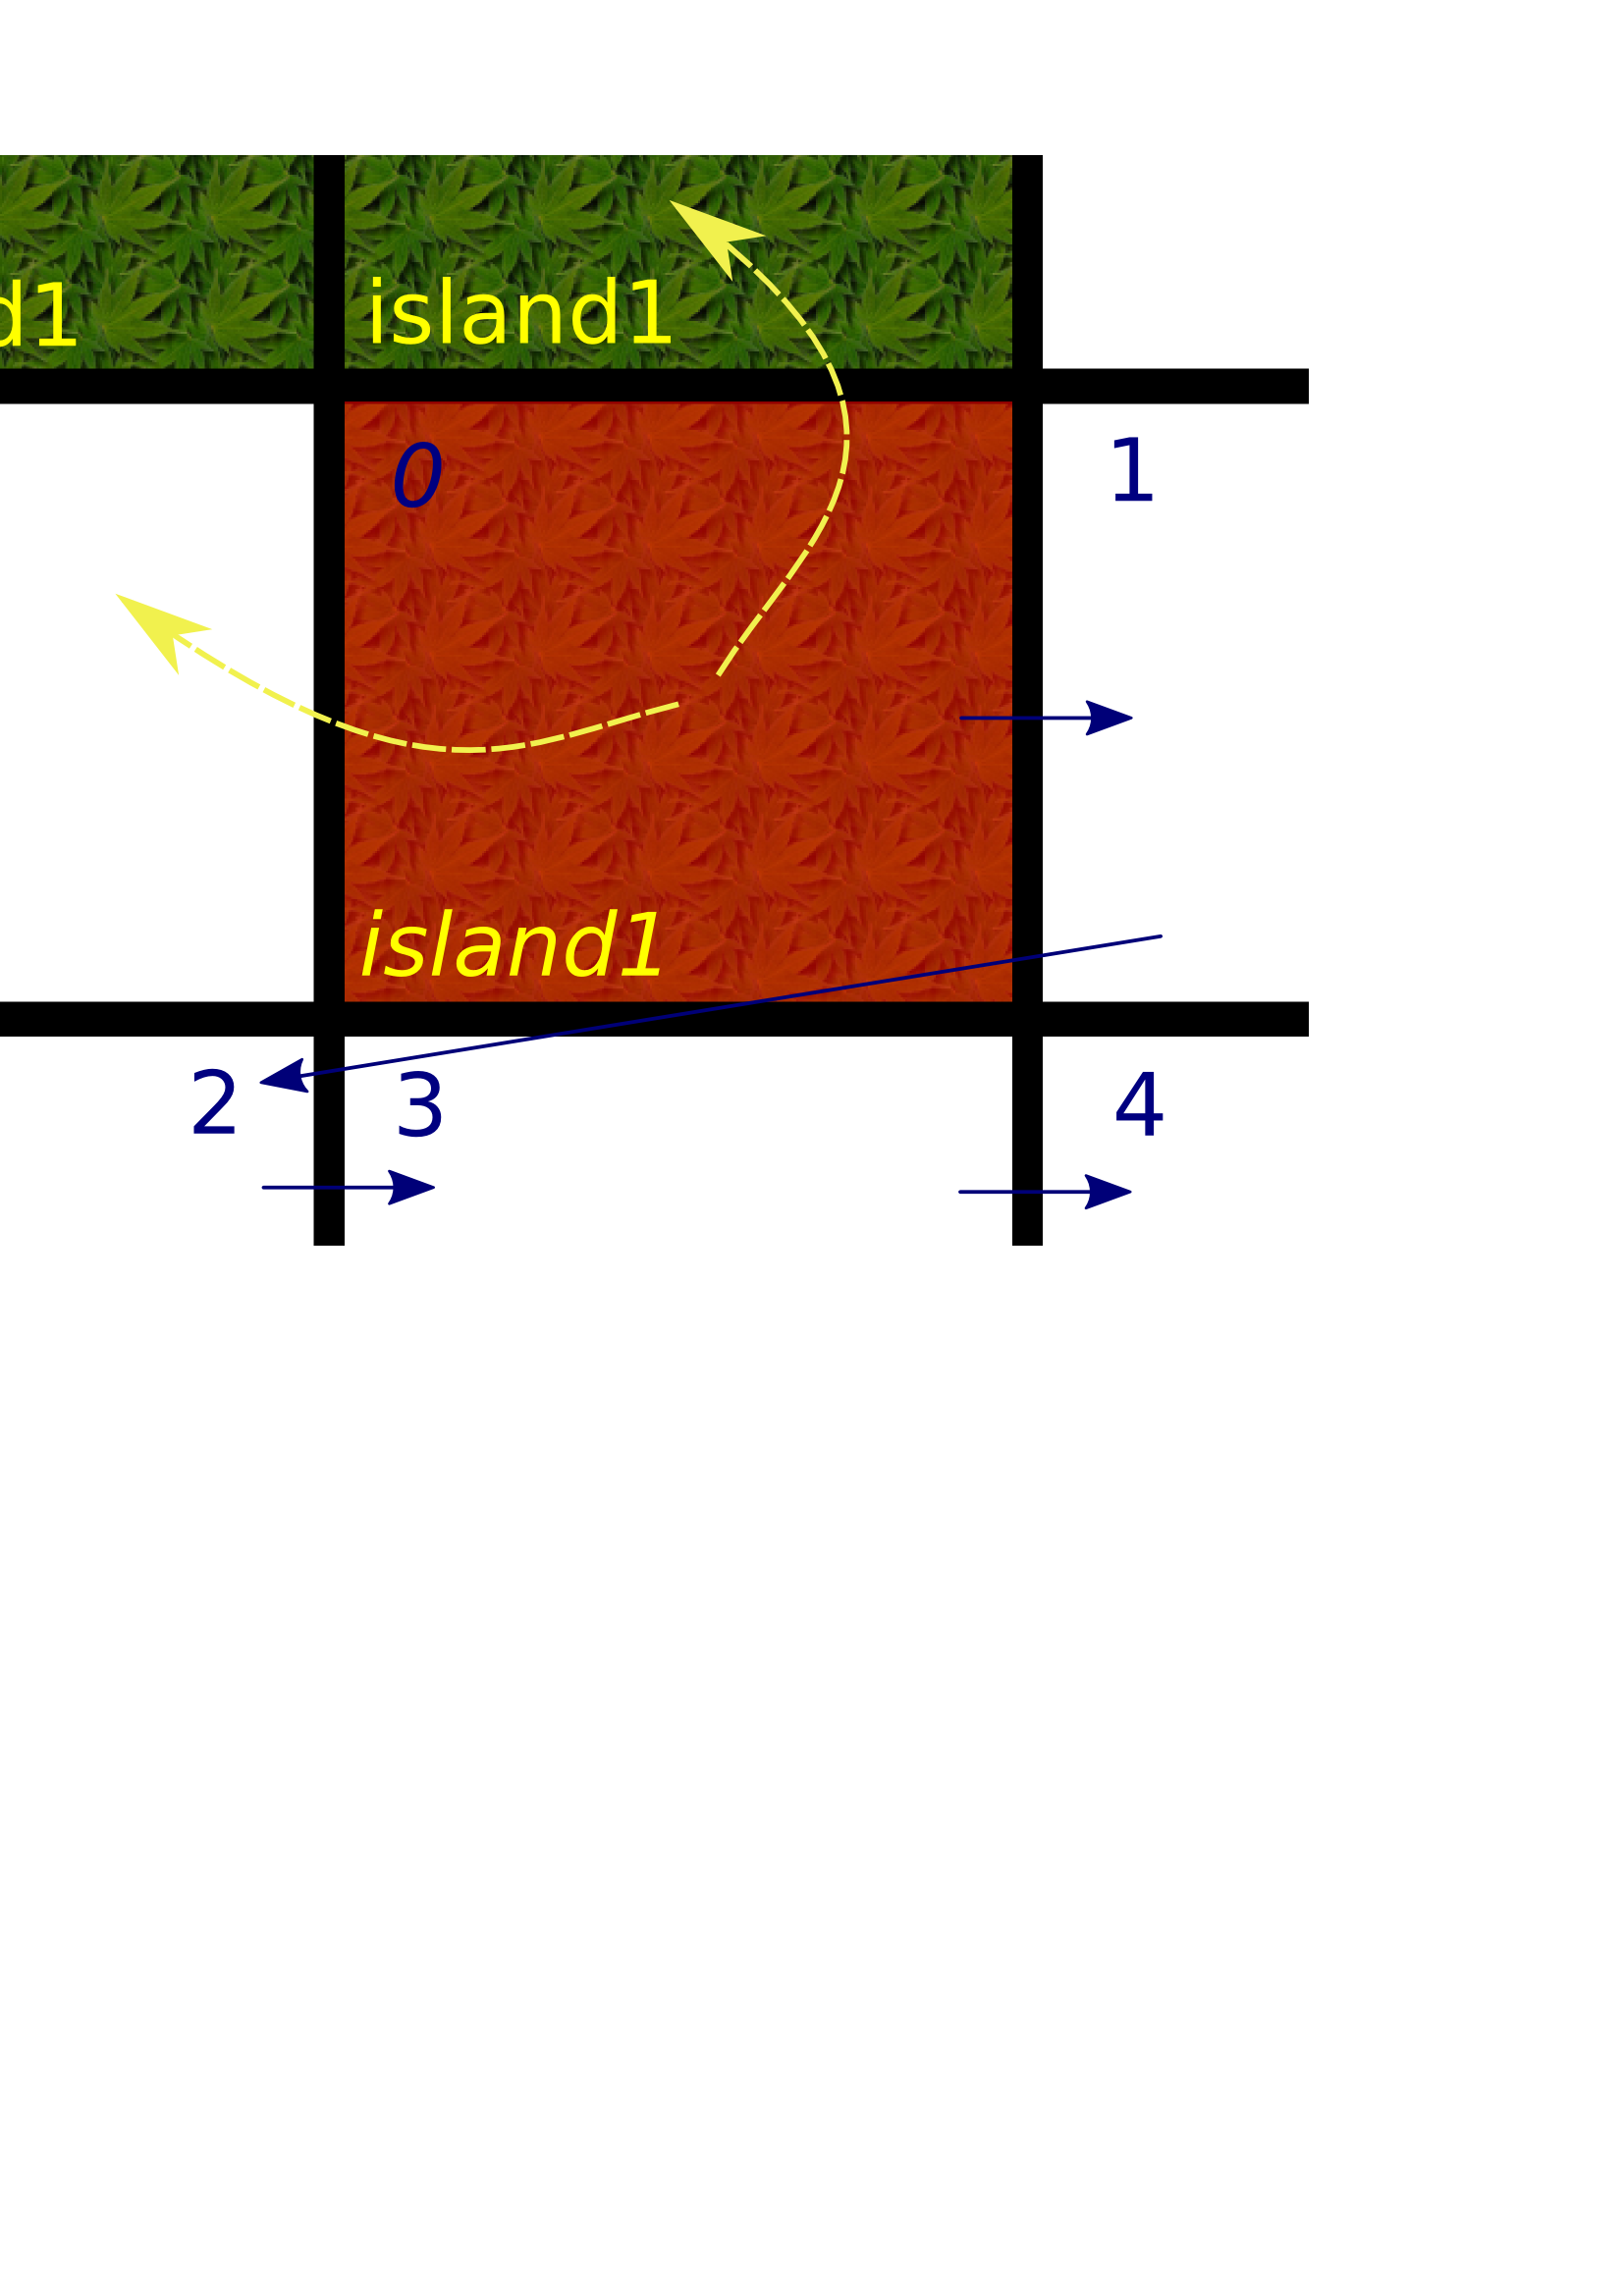
\includegraphics[width=0.7\textwidth]{gfx/Zeichnung.png}
  
  \caption{Der Partitionierungsalgorithmus für die Islands. Die gelben Pfeile
  geben an, welche Gitterflächen auf das Vorhandensein von Tiles überprüft
  werden. Der Algorithmus traversiert die Tiles von oben links nach unten
  rechts (blau eingezeichnet).}
  \label{figure:automaton-intersection}
\end{figure}

Wie in Abschnitt \ref{kartenformat} erklärt, besteht die Schwierigkeit des
Transformationsprozesses in diese Richtung darin, zusammenliegende Bodentiles zu
erkennen. Dadurch benötigt das Speichern großer Inseln eine gewisse Zeit bis die
Gruppierung der Inslen beendet ist.


\section{Vorgehen}
In diesem Kapitel beschreiben wir zunächst, welche grundlegenden Arbeitsprozesse
wir verwendet haben. Anschließend schildern wir den zeitlichen Ablauf des
Projektes.

\subsection{Grundlegende Arbeitsweise und -aufteilung}
Die gesamte anstehende Arbeit wurde in mehrere Unteraufgaben aufgeteilt, die wir
zumeist einzeln erledigten.
In besonderen Fällen wichen wir jedoch auf Pair Programming aus. Wir trafen uns
regelmäßig einmal die Woche, um unseren Fortschritt festzustellen und gemeinsam
am Projekt weiterzuarbeiten. In einer einfachen Textdatei wurden Milestones
definiert und festgelegt, bis wann von wem welche Funktion implementiert sein
sollte (vgl. Bild~\ref{figure:assignee}).

\begin{figure}[htbp]
  \centering

    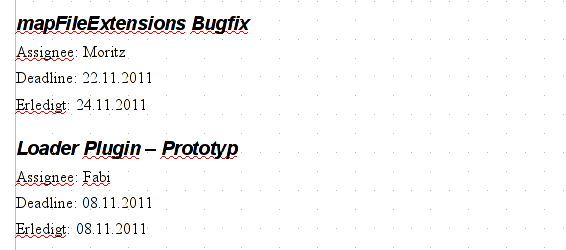
\includegraphics[width=0.4\textwidth]{gfx/assignee.png}

  \caption{Ausschnitt unserer Roadmap.}
  \label{figure:assignee}
\end{figure}

Zu Beginn des Projektes haben wir zunächst mit den UH-Entwicklern gesprochen,
um festzustellen, welche Anforderungen der Editor erfüllen sollte. Hierzu
haben wir uns informell mit einigen der Entwicklern im IRC unterhalten und
festgestellt, dass der bestehende FIFE-Editor eine gute Basis für den Map
Editor darstellt.

Anschließend haben wir uns in den bestehenden Code des Editors und den
Ladeprozess von UH eingelesen, um herauszufinden, welche Schwierigkeiten bei der
Implementierung bestehen könnten und wie eine funktionstüchtige Architektur
aussehen könnte.
In einer kurzen Diskussion im FIFE IRC-Channel haben wir herausgefunden, dass
derzeit am FIFE-Editor gearbeitet wird, um die Integration von anderen
Kartenformaten zu ermöglichen, dass dieser Prozess jedoch noch nicht
abgeschlossen ist. Nach gründlicher Überlegung haben wir damit begonnen,
grundsätzliche Probleme zu identifizieren, bevor wir mit der eigentlichen Arbeit
-- dem Implementieren der Loader und Saver Plugins -- beginnen konnten. Die sich
abzeichnenden Aufgaben strukturierten wir und hielten sie in einer Roadmap fest
(siehe Bild~\ref{figure:assigneeq}).

\subsection{Zeitlicher Ablauf des Projekts}
 Es stellte sich heraus, dass
prinzipiell mit dem Loader-Plugin direkt begonnen werden konnte, das MapSaver
Plugin jedoch einige Vorarbeit an FIFE selbst erforderte. Grundsätzlich fuhren
wir ab da die Entwicklung des MapLoaders und MapSavers Plugin weitgehend
parallel zueinander. Hierzu teilten wir die Arbeit auf, da sich abzeichnete,
dass beides ungefähr gleichen Arbeitsaufwand bedeutete.

Während unserer Arbeit an den Plugins stellten sich einige Unzulänglichkeiten
des FIFE Editors heraus. Um diese zu beheben, schrieben wir etliche Patches für
FIFE, die z.B.
Bugs im Dateiauswahldialog des Editors behoben. Für das Saver-Plugin fehlte die
Infrastruktur-Unterstützung durch FIFE komplett und musste eigens erstellt
werden. Die resultierenden Patches haben wir anschließend in den FIFE Bugtracker
gestellt, von wo sie von einem der FIFE Entwickler gemerged wurden.


Um Laden UH Objekte zu laden, war eine weitere intensive Beschäftigung mit dem
FIFE Editor Code und dem UH Kartenformat nötig. Solbald die Objekte im Editor
geladen werden konnten, präsentierten wir unseren Fortschritt in einem der
wöchentlichen Meetings von UH.

Da zu dieser Zeit gerade größere Umbauarbeiten an der Architektur des Spiels vorgenommen wurden,
kam es zu einem Konflikt mit unserem Editor-Code. Änderungen am Spiel zwangen uns, einen Teil
des Codes neu zu schreiben, um mit den neuen Features des Spiels kompatibel zu bleiben. Dies
hätte allerdings nicht vermieden werden können, da die Änderungen bereits vor dem Beginn des
Editor-Projekts geplant waren und nicht verschoben werden konnten. Da wir bereits frühzeitig
auf einem weiter fortgeschrittenen Branch des Git-Repositories gearbeitet hatten, war der
Umfang der nötigen Änderungen noch angemessen.


Parallel trieben wir die Entwicklung des MapSavers voran. Wir begannen damit,
zunächst nur Buildings abzuspeichern, da dies wesentlich einfacher war, als
Groundtiles. Die resultierenden Karten zeigten im Nichts hängende Gebäude, was
jedoch schon ein großer Fortschritt war.
Anschließend kümmerten wir uns um das Abspeichern der Groundtiles. Dies
erforderte das Erstellen eines Partitionierungsalgorithmus, der zusammengehörige
Tiles automatisch erkennt und zu einer Insel gehörig abspeichert.

Ein großer Punkt war jedoch zu diesem Zeitpunkt noch offen: Die Rotation von
Objekten auf der Karte.
Bisher lud der MapLoader die Objekte noch ohne Rotation, sie zeigten folglich
alle in die gleiche Richtung. Auch der MapSaver speicherte keine Rotationsdaten.
Nach einiger Recherche und ein paar erfolglosen Versuchen, die Rotation der
Gebäude richtig zu setzen, wandten wir uns an die UH-Entwickler.
Wie sich herausstellte war der Code-Abschnitt, der im Spiel die Gebäude rotiert
relativ alt und niemand konnte sich mehr erinnern, wie er funktioniert
(Original-Kommentar ``nobody actually knows how the code below works.'').
Es gab auch keine Dokumentation zu diesem Punkt. Leider stolperten wir sehr oft
über genau diesen Code.

Daraufhin entschlossen wir uns, das Problem in einer Pair-Programming-Sitzung anzugehen. Dies hatte
den Vorteil, dass wir das Problem gleichzeitig und mit zwei unterschiedlichen Sichtweisen betrachten
konnten, während wir zusammen aktiv an einer Lösung arbeiteten. Hierdurch gelang es uns, eine funktionierende
Rotation der Objekte im MapLoader zu implementieren.

Über die Weihnachtszeit erfolgte dann ein weiterer großer Umbau der Architektur
von UH. Das gesamte Design aller auf der Karte platzierten Objekte wurde
umgestellt, woraufhin unser Edior-Code zunächst nicht mehr funktionstüchtig war.
Nach einem vollen Tag an Arbeit waren die Plugins jedoch wieder einsatzfähig.


Schlussendlich wurde durch ein FIFE-Update das Rückgeben von Koordinatenwerten
im Editor ungenau: Statt $[45^\circ, 135^\circ, 225^\circ, 315^\circ]$ wurden
nun Werte wie $44^\circ, 46^\circ$ etc. von der {\tt getRotation()}-Methode des
Editors zurückgegeben. Da UH grundsätzlich gegen den FIFE trunk kompiliert wird,
mussten wir hierfür zusätzlich eine Korrekturfunktion schreiben. Allein das
Debugging nahm Stunden in Anspruch.



\section{Erfahrungen}
Im Zuge des Praktikums haben wir sowohl positive als auch negative Erfahrungen
gemacht. Diese legen wir im Folgenden dar.

\subsection{Positive Erfahrungen}
Grundsätzlich gesteltate sich die Zusammenarbeit mit den anderen Beteiligten
des UH Projekts als äußerst locker und einfach. Durch die ständige Anwesenheit
von Personen im IRC Channel und die Aufgeschlossenheit, Hilfsbereitschaft und
Geduld der Entwickler des UH Teams wurde unsere Arbeit deutlich erleichtert,
sei es beim Verstehen komplizierter Zusammenhänge und Vorgänge oder beim
finden von Fehlern in unserem Code.

Durch die regelmäßigen sonntäglichen Treffen wurde eine einfache
Kommunikatiosplattform geschaffen, über die wir unsere Ergebnisse kommunizieren
und Feedback aus der Entwicklergemeinde einholen konnten. Dies führte dazu,
dass unser Projekt innerhalb eines akzeptablen Rahmens blieb und gleichzeitig
vom UH Team ohne große Probleme übernommen wurde.

Ein weiterer Punkt, der hierzu beigetragen hat ist die Tatsache, dass der Editor
Code vom restlichen Code des Spiels in großen Teilen unabhängig ist.
Hierdurch waren wir auch durch große Änderungen am Spiel selbst nur mäßig
betroffen und konnten unser Projekt unabhängig von der Entwicklung des Spiels
selbst gestalten. Daraus resultierend kam es während der gesamten Entwicklung zu
keinem einzigen Merge-Konflikt und die einzigen Änderungen am Spiel, die
Auswirkungen auf unseren Code hatten, waren groß angelegte Refactorings der
Architektur. Hier war der Zeitpunkt für die Editorerstellung ungünstig.

\subsection{Negative Erfahrungen}
Es gab jedoch auch Probleme bei der Umsetzung unseres Vorhabens.
So gingen die oben genannten Änderungen an der Spielarchitektur nicht spurlos
an uns vorbei. Es waren einige Anpassungen nötig, wie in den vorangegangenen Kapiteln
beschrieben, um unseren Editor-Code wieder funktionstüchtig zu machen.
Diese Umstellung der Architektur wurden uns leider nicht ausführlich genug
kommuniziert, wahrscheinlich auch deshalb, weil keinem der Entwickler klar war,
dass dies auch Auswirkungen auf unseren Code haben könnte.

Des weiteren änderte sich einmal während der Entwicklungszeit das Format der
Maps geringfügig, wodurch einige Anpassungen in unserem Loader und Saver vonnöten
waren. Auch hier wurde uns vorher keine Mitteilung gemacht.

Schließlich gab es noch einige kleinere Stolpersteine, die dadurch entstanden,
dass wir nicht nur für UH gearbeitet haben, sondern teilweise auch Code
für das FIFE Projekt geschrieben haben, da wir deren Editor verwendeten.
Dies bedingte, dass wir doppelten Koordinationsaufwand hatten: Zum einen mit
den UH Entwicklern und zum andern mit dem FIFE Team.

Schlussendlich wurde durch ein FIFE-Update das Rückgeben von Koordinatenwerten
im Editor ungenau: Statt $[45^\circ, 135^\circ, 225^\circ, 315^\circ]$ wurden
nun Werte wie $44^\circ, 46^\circ$ etc. von der {\tt getRotation()}-Methode des
Editors zurückgegeben.
Da UH grundsätzlich gegen den FIFE trunk kompiliert wird, mussten wir hierfür
zusätzlich eine Korrekturfunktion schreiben. Allein das Debugging nahm Stunden
in Anspruch.

\subsection{Schlüsse}
Aus den gemachten Erfahrungen konnten wir einige Lehren ziehen, die nicht nur
für uns selbst, sondern auch für zukünftige Teams des Open-Source-Praktikums
von Interesse sind.

\subsubsection{Aktives Nachfragen}
Um die Koordination mit den Entwicklern des Open Source Projekts zu verbessern,
hilft es, eigenständig Nachfragen anzustellen. Fragen wurden in
unserem Projekt stets mit Hilfsbereitschaft aufgenommen. Hierdurch ist es möglich,
Probleme schneller zu lösen. Auch können so zukünftige Konflikte vermieden werden,
etwa wenn größere Änderungen geplant sind. Da die Entwickler oft keinen guten
Einblick in das bearbeitete Thema haben, ist ihnen oft nicht klar, ob ihre eigenen
Entscheidungen Konsequenzen für das Projekt haben. Eine kurze Nachfrage, ob die
geplante Änderung relevante Codeteile betrifft hilft, einfach Klarheit zu schaffen
und Vorbereitungen für die anstehenden Änderungen zu treffen.

\subsubsection{Klare Abgrenzung}
Eine klare Abgrenzung des geplanten Features vom Rest des Open Source Projekts
erleichtert eine Koordination mit anderen Entwicklungsmaßnahmen und verhindert
Konflikte und Integrationsprobleme. In unserem Fall war nicht nur der Code
größtenteils unabhängig vom Hauptprojekt, er wurde sogar in einer eigenen
Verzeichnisstruktur abgelegt.

\subsubsection{Bedürfnis erfüllen}
Das wichtigste bei der Auswahl eines guten Projektes ist die Relevanz des
bearbeiteten Themas und das Bedürfnis des Projekts für das erstellte Feature.
In unserem Fall wird der Map-Editor dringend gebraucht. Dies bedeutet, dass
unsere Implementierung auf jeden Fall angenommen wird, auch wenn noch Defizite
in der Umsetzung bestehen.



\bibliography{paper}{}
\end{document}

